\documentclass[xcolor={usenames,dvipsnames},hyperref={unicode}]{beamer}

\usepackage{latexsym,amssymb,amsmath,amsbsy,amsopn,amstext,color,multicol}
\usepackage{graphicx,wrapfig,fancybox,watermark,picins}
\usepackage{pgf,pgfarrows,pgfnodes,pgfautomata,pgfheaps,pgfshade}
\usepackage{CTex}
\setbeamercovered{transparent}

\definecolor{beamer@blendedblue}{rgb}{0.109803922,0.325490196,0.545098039}
\setbeamercolor{structure}{fg=beamer@blendedblue}

\setbeamertemplate{caption}[numbered]
\usetheme{Frankfurt}

\setbeamercolor{alerted text}{fg=Maroon}
\setbeamertemplate{items}[square]
\setbeamertemplate{frametitle}[default][colsep=-4bp,rounded=false,shadow=false]

\makeatletter
\setbeamertemplate{headline}
{%
	\pgfuseshading{beamer@barshade}%
	\ifbeamer@sb@subsection%
		\vskip-9.75ex%
	\else%
		\vskip-7ex%
	\fi%
	\begin{beamercolorbox}[ignorebg,ht=2.25ex,dp=3.75ex]{section in head/foot}
    	\insertnavigation{0.95\paperwidth} % <======= Added 0.5 here
	\end{beamercolorbox}%
	\ifbeamer@sb@subsection%
    \begin{beamercolorbox}[ignorebg,ht=2.125ex,dp=1.125ex,%
		leftskip=.3cm,rightskip=.3cm plus1fil]{subsection in head/foot}
		\usebeamerfont{subsection in head/foot}\insertsubsectionhead
    \end{beamercolorbox}%
	\fi%
}%

\begin{document}

\title{遗传算法 \& 模拟退火} %题目,把这块改成演讲题目
\author{杨亚龙}
\institute{天津大学}
\date{2014-04-01}
\pgfdeclareimage[width=1.2cm,height=1.2cm]{logo}{logo}
\logo{\pgfuseimage{logo}}

\AtBeginSection[]{\frame{\frametitle{Outline}\tableofcontents[current]}}
\frame{\titlepage}

\part{Main Part}
\frame{\frametitle{Outline}\tableofcontents[part=1]}

\section{遗传算法}
\subsection{初衷和流程}
\frame{
	\frametitle {\secname - \subsecname}
	\begin{block}{初衷}
	模拟生物进化理论,优胜劣汰,不断进步,产生更优分类器。
	\end{block}
	\begin{block}{流程}
		\begin{enumerate}
			\item 生成若干个分类器(互相不一样)
			\item 完成有label的分类任务,并评价任务结果
			\item 保留部分排名靠前的
			\item 随机两两“变异”这些留下来的分类器,在进行2-4步骤,直到满足性能要求
		\end{enumerate}
	\end{block}
}
\subsection{两大问题}
\subsubsection{如何表示分类器}
\frame{
	\frametitle {\subsubsecname - 二进制串表示}
	\begin{itemize}
		\item 将分类器encode和decode成二进制串的过程
		\item 例如:二叉决策树,每次决策的条件都可编码成二进制。如符号、比较数等
	\end{itemize}
}

\frame{
	\frametitle {\subsubsecname - 基于计算机程序片段}
	\begin{itemize}
		\item 将分类器encode和decode成有文法意义的串的过程,如主谓宾,谓语后面只能接名词
		\item 我觉得可以理解成比二进制串更加多限制的表示形式,能更加精确描述分类器
	\end{itemize}
}


\subsubsection{如何“变异”}
\frame{
	\frametitle {\subsubsecname}
	发生在两两之间
	\begin{itemize}
		\item 复制
			\begin{itemize}
				\item 两个不变
			\end{itemize}
		\item 交叉
			\begin{itemize}
				\item 随机选择一个位置,从此位置截断,互相换
				\item 如:111000 与 000111 交叉,如果随机到了3位置,则结果为 111111 和 000000
			\end{itemize}
		\item 变异
			\begin{itemize}
				\item 对于二进制串,每一位以一定的概率(通常较小),0变1,1变0
				\item 对于程序片段,每个元素可以以另一个同类元素替换
			\end{itemize}
		\item 插入
			\begin{itemize}
				\item 一般发生在程序片段中,每个元素可以以另一个片段替换,要符合文法
			\end{itemize}
	\end{itemize}
}

\subsection{其他一些需要注意的问题}
\frame{
	\frametitle {\subsecname}
	\begin{itemize}
		\item 对分类器打分,通常以一个对分类正确率单调的函数
		\item 防止过拟合的通常做法
			\begin{itemize}
				\item 对分类器过于复杂的进行惩罚(基于一般简单的更好的想法)
				\item 设计好的停止准则(以经验为主)
			\end{itemize}
		\item 启发式进行;主要指根据每一代的平均得分情况,动态改变\textbf{变异率和交叉率}
		\item 不完全按照打分排序来选择,而采用一个正比于打分,同时有一个控制因素的
			\begin{itemize}
				\item $P(i) = \frac{e^{f_i/T}}{\varepsilon[e^{f_i/T}]}$
				\item 可以描述着一个种群,进化早期,所有个体都有计划被选择;进化后期则保持特异性,小范围集中搜索
			\end{itemize}
	\end{itemize}
}

\subsection{优缺点}
\frame{
	\frametitle {\subsecname}
	\begin{itemize}
		\item 优点
			\begin{itemize}
				\item 适用于并行计算,每个分类器进行分类打分过程完全独立
				\item 通常变异过程对分类器变化很大,所以不容易跳入局部最优;原文:能在“极复杂的非连续空间”和“适应度地形曲面”也能有很好的解
			\end{itemize}
		\pause
		\item 缺点
			\begin{itemize}
				\item 无法进行理论表述
				\item 与领域相关性,经验相关性很大。如,如何表述分类器,如何设置变异率等。
			\end{itemize}
		\item 总结by作者:随着计算费用下降,模式分类问题将更多依赖于计算能力,而不是精巧的分类器设置,这种情况下,随机搜索算法很有前途
	\end{itemize}
}

\section{模拟退火}
\frame{
	\frametitle {爬山问题}
	\begin{figure}
		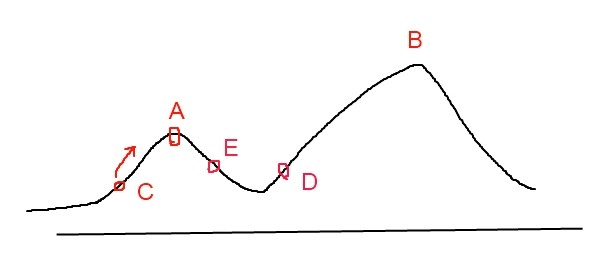
\includegraphics[scale=0.5]{pic/tuihuo}
		\caption{爬山问题}
	\end{figure}
}

\frame{
	\frametitle {模拟退火解决}
	\begin{itemize}
		\item 每次有一定机会不朝最高点爬
		\item 这个“一定机会”(也就是概率)随着时间推移减少,这也称为金属退火过程
	\end{itemize}
}

\frame{
	\frametitle {Thank you}
	Thank you for listening !
}

\end{document}